% rsl_manuscript.tex -- Remote Sensing Letters submission (Taylor & Francis Interact layout, Chicago author-date)
\documentclass[]{interact}

\usepackage{graphicx}
\usepackage{booktabs}
\usepackage{multirow}
\usepackage{amsmath,bm}
\usepackage{tikz}
\usetikzlibrary{arrows.meta, positioning}
\usepackage{url}

\usepackage{natbib}% Citation support using natbib.sty
\bibpunct[, ]{(}{)}{;}{a}{}{,}
\renewcommand\bibfont{\fontsize{10}{12}\selectfont}

\graphicspath{{results/figures/}}
\newcommand{\pp}{\,pp}

\begin{document}

\articletype{LETTER}

\title{Annotation budget and inductive bias: deep learning versus gradient boosting for hyperspectral classification under spatially disjoint evaluation}

\author{
\name{Swati Hira\textsuperscript{a}\thanks{CONTACT Swati Hira. Email: shira@iiitn.ac.in}, Devguru Tiwari\textsuperscript{a}, Nagamani Molakatala\textsuperscript{b}, R. Kokila\textsuperscript{c}, Gururaja H S\textsuperscript{d} and J. Rajini\textsuperscript{e}}
\affil{\textsuperscript{a}Department of Computer Science and Engineering, Indian Institute of Information Technology, Nagpur, Maharashtra, India; \textsuperscript{b}School of Computer and Information Sciences, University of Hyderabad, Hyderabad, Telangana, India; \textsuperscript{c}School of Computer Applications, Dayananda Sagar University, Bengaluru, Karnataka, India; \textsuperscript{d}Department of Computer Science and Business Systems, B.M.S. College of Engineering, Bangalore, Karnataka, India; \textsuperscript{e}Department of English, Kongu Engineering College, Erode, Tamil Nadu, India}
}

\maketitle

\begin{abstract}
Labels for hyperspectral classification are expensive, so classifiers are often trained on a few per cent of the pixels. We compare LightGBM with four deep models (a spectral transformer, a grouped-band transformer, a conv-stem transformer and the 3-D CNN HybridSN) on three airborne scenes (Indian Pines, Pavia University, Salinas) with spatially disjoint training and test areas, and on a laboratory dataset of Indian soils evaluated on held-out physical samples. All models share one protocol and five paired seeds; tests are corrected for multiple comparisons. The result depends on the scene and on inductive bias. HybridSN is 3--9 percentage points (pp) more accurate than LightGBM at every budget on Pavia University and Salinas (0.5--5\% labelled pixels) and, on the soil data, significantly more accurate with four labelled samples per class (+8.8\pp). On Indian Pines no deep model is significantly better than LightGBM. The two transformers that see only the centre-pixel spectrum are never significantly better than LightGBM. Cross-domain pre-training gives no gain that survives correction, and it lowers the accuracy of the spectral transformer on Indian Pines.
\end{abstract}

\begin{keywords}
Hyperspectral imaging; annotation budget; LightGBM; transformer; spatially disjoint split; soil classification
\end{keywords}

\section{Introduction}
Hyperspectral imaging (HSI) records hundreds of narrow spectral bands and is used for agricultural and soil surveys \citep{Bioucas2013}. Labelling is the costly part: soil classes require field sampling and laboratory analysis, so classifiers are usually trained with a small share of labelled pixels.

Deep models, including 3-D convolutional networks \citep{Zhong2018,Roy2020}, graph convolutional networks \citep{Hong2021} and transformers \citep{Hong2022}, report high accuracy on public benchmarks. Two caveats apply. Transformers need much data unless an inductive bias is built in \citep{Hassani2021}, while gradient-boosted trees remain strong on tabular input \citep{Ke2017,Grinsztajn2022}, and a hyperspectral pixel is a tabular vector. Moreover, the usual random pixel split lets training and test patches overlap, which inflates patch-based models \citep{Nalepa2019}.

We therefore ask, under spatially disjoint evaluation, at which annotation budget a deep model becomes more accurate than LightGBM. Our contributions are: (i) one protocol (disjoint training and test areas, shared preprocessing, five paired seeds, false-discovery-rate control) applied to LightGBM and four deep models on three airborne scenes and one laboratory soil dataset; (ii) for the soil data, budgets counted in labelled physical samples rather than patches; (iii) a transfer study in both directions between an airborne scene and the soil images; and (iv) TreeSHAP band importance \citep{Lundberg2020} at the true band-centre wavelengths.

\section{Data}\label{sec:data}

\emph{Airborne scenes.} Indian Pines (AVIRIS; $145\times145$ pixels, 200 bands after water-band removal, 16 classes, 10\,249 labelled pixels), Pavia University (ROSIS; $610\times340$ pixels, 103 bands, 9 classes, 42\,776 labelled pixels) and Salinas (AVIRIS; $512\times217$ pixels, 204 bands, 16 classes, 54\,129 labelled pixels). Indian Pines band centres are taken from the 1992 AVIRIS calibration distributed with the scene; after water-band removal they are not monotonic in band index.

\emph{Local Indian soil.} Soil samples from agricultural regions of Maharashtra, Gujarat and Hisar (Haryana), provided by the NBSS, were imaged in the laboratory with a Resonon Pika NIR-320 line-scan camera (320 spatial pixels, 168 bands, 888.7--1714.6\,nm according to the image headers). We use the Black, Red and Yellow soil folders: 36 images of 24 physical samples (7, 10 and 7 per class). The 11 images of mixed soils have no single label and are excluded. Each image is cut into non-overlapping $15\times15$ patches. Soil type is partly confounded with moisture and acquisition date: all Black-soil images were acquired moist, all Yellow-soil images dry, and Red soil in both states.

\section{Methods}\label{sec:methods}

\begin{figure}
\centering
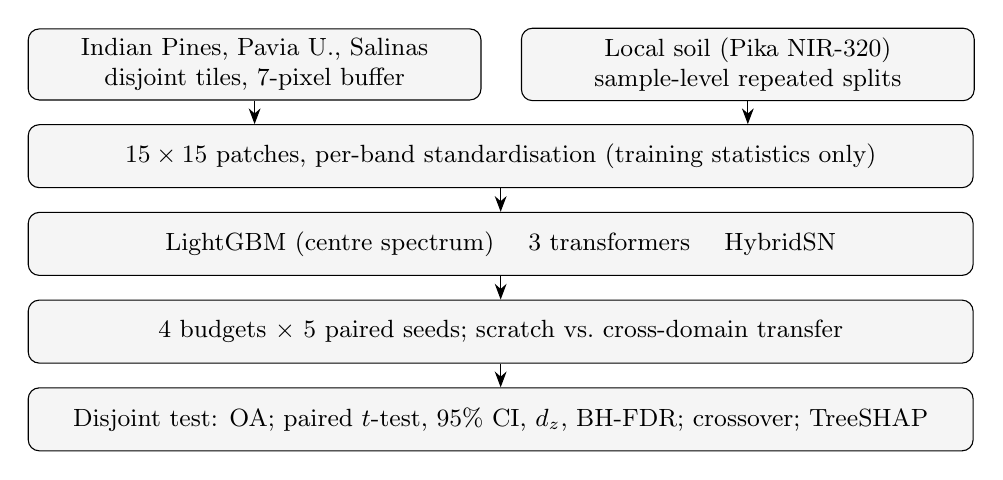
\begin{tikzpicture}[node distance=3mm, every node/.style={font=\small, align=center},
  box/.style={draw, rounded corners, minimum height=8mm, fill=gray!8},
  arr/.style={-{Stealth[length=2mm]}}]
\node[box, minimum width=5.75cm] (ip) {Indian Pines, Pavia U., Salinas\\ disjoint tiles, 7-pixel buffer};
\node[box, minimum width=5.75cm, right=5mm of ip] (ls) {Local soil (Pika NIR-320)\\ sample-level repeated splits};
\node[box, minimum width=12cm, below=of ip, xshift=3.125cm] (pre) {$15\times15$ patches, per-band standardisation (training statistics only)};
\node[box, minimum width=12cm, below=of pre] (mod) {LightGBM (centre spectrum) \quad 3 transformers \quad HybridSN};
\node[box, minimum width=12cm, below=of mod] (bud) {4 budgets $\times$ 5 paired seeds; scratch vs.\ cross-domain transfer};
\node[box, minimum width=12cm, below=of bud] (ev) {Disjoint test: OA; paired $t$-test, 95\% CI, $d_z$, BH-FDR; crossover; TreeSHAP};
\draw[arr] (ip) -- (ip|-pre.north); \draw[arr] (ls) -- (ls|-pre.north);
\draw[arr] (pre) -- (mod); \draw[arr] (mod) -- (bud); \draw[arr] (bud) -- (ev);
\end{tikzpicture}
\caption{Experimental workflow.}
\label{fig:workflow}
\end{figure}

\subsection{Models}
All deep models receive a $15\times15$ patch (Figure~\ref{fig:workflow}). \textbf{LightGBM} \citep{Ke2017} uses the centre-pixel spectrum with 100 trees and default settings except \texttt{max\_delta\_step}$=1$, which caps each leaf's output; without it, training diverged on one Salinas split. The \textbf{spectral transformer} sees only the centre pixel, with one token per band (128-d, 4 layers, 4 heads, mean pooling). The \textbf{grouped-band transformer}, inspired by SpectralFormer \citep{Hong2022}, also sees only the centre pixel; each token holds four adjacent bands (64-d, 4 pre-norm layers, learnable cross-layer fusion). On Pavia University the last 3 of 103 bands do not fill a group and are dropped. The \textbf{conv-stem transformer} is the spectral transformer with band tokens produced by two 3-D convolutions over the whole patch, which isolates the effect of a local inductive bias. \textbf{HybridSN} \citep{Roy2020} has three 3-D convolutions, one 2-D convolution and two dense layers.

\subsection{Evaluation protocol}\label{sec:protocol}
\emph{Airborne scenes.} Each scene is divided into square tiles (24 pixels for Indian Pines, 32 for the others), and half of the tiles form the training area. For each seed, the best of 400 random assignments is kept, ranked first by the number of classes with a fair share in both halves ($\ge$25\% of the class in the training area and $\ge$10\% in the test area). Test pixels within 7 pixels of a training tile are dropped, so no test window contains a training-area pixel. Training pixels are drawn from the training area per class, in proportion to its class frequencies, to a total of $p$ of all labelled pixels ($p\in\{1,5,10,20\}\%$ for Indian Pines, $\{0.5,1,2,5\}\%$ for the larger scenes). Up to 3\,000 further training-area pixels form the validation set, which is used only for early stopping. Only classes present in the training area are scored: 9 of 9 on Pavia University, 16 of 16 on Salinas, and 10--13 of 16 on Indian Pines, whose small fields cannot all be split. Test areas contain 2\,594--3\,560 (Indian Pines), 16\,173--17\,500 (Pavia University) and 17\,802--18\,986 (Salinas) pixels, depending on the seed; the test area is fixed per seed across budgets.

\emph{Local soil.} Images of one physical sample share a sample number and are never split. For each of five repeats, the samples of each class are shuffled: 2 go to the test set, 1 to the validation set, and the budget $k\in\{1,2,3,4\}$ is the first $k$ of the remaining samples per class (nested). Patches of one sample are near-duplicates, so at most 300 per training or validation sample are used; the test set uses every patch (5\,460--5\,628).

\emph{Training.} All deep models use AdamW (learning rate $5\times10^{-4}$, weight decay $10^{-4}$), cosine annealing, batch size 64 and at most 50 epochs with early stopping (patience 10) on validation loss, restoring the best weights. Inputs are standardised per band with training statistics. Models and LightGBM use the same splits per seed, so comparisons are paired. Runs used PyTorch 2.11, CUDA 12.8 and LightGBM 4.6 on Kaggle (NVIDIA Tesla T4 for the deep models).

\emph{Transfer.} Source models are trained on all Local soil samples except one validation sample per class, or on all labelled Indian Pines pixels (10\% for validation). Every target tensor whose name and shape match the source is copied, except the classifier, and positional embeddings are linearly resampled along the band axis (168 versus 200 bands). Copied layers are frozen for 5 epochs, after which the whole network is trained at a learning rate of $1\times10^{-4}$. The sensors cover different wavelengths (400--2500\,nm versus 889--1715\,nm), so the resampling matches band order, not wavelength.

\emph{Statistics.} For each comparison we report the mean paired difference over the five seeds, its 95\% confidence interval, Cohen's $d_z$ and the paired $t$-test $p$-value adjusted with the Benjamini--Hochberg procedure (reported as $q$). We correct within three families: (1) every model-versus-LightGBM test on the airborne scenes (48 tests), (2) every model-versus-LightGBM test on Local soil (16 tests), and (3) every transfer-versus-scratch test in both directions (24 tests). The \emph{crossover} is the budget after which a model's mean accuracy stays above that of LightGBM, found by linear interpolation; its 95\% interval comes from 5\,000 resamples of the seeds.

\section{Results}\label{sec:results}

\subsection{Airborne scenes}
Table~\ref{tab:scenes} and Figure~\ref{fig:scenes} give overall accuracy (OA) on the disjoint test areas. On Pavia University and Salinas, HybridSN is the most accurate model at every budget, 6.9--9.1\pp\ above LightGBM on Pavia University and 3.1--8.2\pp\ on Salinas; five of these eight differences are significant ($q\le0.04$). The conv-stem transformer is above LightGBM on Pavia University from 0.5\% (+2.4 to +6.8\pp) and on Salinas from about 1\% (crossover 0.8\%, 95\% CI 0.5--1.2\%), significantly so at 2\% on both scenes and at 5\% on Salinas. The two centre-pixel transformers are at or below LightGBM throughout. The grouped-band transformer is significantly below it on Pavia University at 2\% and 5\% ($-5.5$ and $-3.9$\pp).

Indian Pines is different. Under the disjoint split all models reach only 31--51\% OA, and no deep model is significantly more accurate than LightGBM at any budget. Both centre-pixel transformers are significantly below it at 5\% ($-9.3$ and $-11.3$\pp, $q\le0.04$). Only the spectral transformer at 20\% has a higher mean than LightGBM ($+2.4$\pp, $q=0.34$).

\begin{table}
\tbl{Overall accuracy (\%) on spatially disjoint test areas (mean $\pm$ SD over 5 seeds).}
{\resizebox{\textwidth}{!}{\begin{tabular}{llccccc}
\toprule
Scene & Labelled & LightGBM & Spectral tr. & Grouped-band tr. & Conv-stem tr. & HybridSN \\
\midrule
\multirow{4}{*}{Indian Pines}
 & 1\% & $\mathbf{37.38 \pm 6.49}$ & $32.90 \pm 9.14$ & $35.15 \pm 9.97$ & $33.01 \pm 9.29$ & $34.95 \pm 7.86$ \\
 & 5\% & $\mathbf{46.90 \pm 5.31}$ & $37.57 \pm 7.71$\textsuperscript{a} & $35.56 \pm 8.67$\textsuperscript{a} & $31.10 \pm 16.36$ & $42.26 \pm 7.84$ \\
 & 10\% & $\mathbf{46.84 \pm 5.56}$ & $42.52 \pm 5.98$ & $40.03 \pm 6.57$ & $37.89 \pm 10.12$ & $43.25 \pm 10.61$ \\
 & 20\% & $48.99 \pm 6.23$ & $\mathbf{51.36 \pm 5.56}$ & $48.03 \pm 5.24$ & $40.95 \pm 10.70$ & $45.16 \pm 6.43$ \\
\midrule
\multirow{4}{*}{Pavia Univ.}
 & 0.5\% & $72.34 \pm 3.97$ & $70.69 \pm 2.85$ & $70.10 \pm 2.48$ & $74.78 \pm 5.12$ & $\mathbf{80.71 \pm 5.60}$\textsuperscript{a} \\
 & 1\% & $74.22 \pm 5.83$ & $72.04 \pm 6.56$ & $71.80 \pm 5.49$ & $79.90 \pm 4.70$ & $\mathbf{83.36 \pm 3.03}$ \\
 & 2\% & $79.15 \pm 2.98$ & $77.69 \pm 5.24$ & $73.69 \pm 2.88$\textsuperscript{a} & $85.94 \pm 4.95$\textsuperscript{a} & $\mathbf{86.01 \pm 5.53}$ \\
 & 5\% & $83.04 \pm 3.57$ & $83.21 \pm 5.07$ & $79.12 \pm 3.09$\textsuperscript{a} & $87.36 \pm 4.99$ & $\mathbf{90.17 \pm 4.41}$\textsuperscript{a} \\
\midrule
\multirow{4}{*}{Salinas}
 & 0.5\% & $73.59 \pm 2.97$ & $64.97 \pm 7.18$ & $69.55 \pm 5.77$ & $70.28 \pm 2.96$ & $\mathbf{76.67 \pm 2.55}$ \\
 & 1\% & $77.77 \pm 3.08$ & $72.77 \pm 3.63$ & $74.92 \pm 2.42$ & $79.85 \pm 3.83$ & $\mathbf{85.97 \pm 3.00}$\textsuperscript{a} \\
 & 2\% & $80.30 \pm 1.47$ & $78.13 \pm 3.99$ & $78.02 \pm 0.87$ & $83.04 \pm 1.21$\textsuperscript{a} & $\mathbf{87.19 \pm 3.36}$\textsuperscript{a} \\
 & 5\% & $81.91 \pm 1.79$ & $81.49 \pm 2.33$ & $81.28 \pm 2.46$ & $86.59 \pm 1.14$\textsuperscript{a} & $\mathbf{89.03 \pm 1.22}$\textsuperscript{a} \\
\bottomrule
\end{tabular}}}
\tabnote{Labelled = share of all labelled pixels used for training; tr. = transformer. \textsuperscript{a}Paired difference from LightGBM significant after BH-FDR over the 48 scene tests ($q<0.05$).}
\label{tab:scenes}
\end{table}

\begin{figure}
\centering
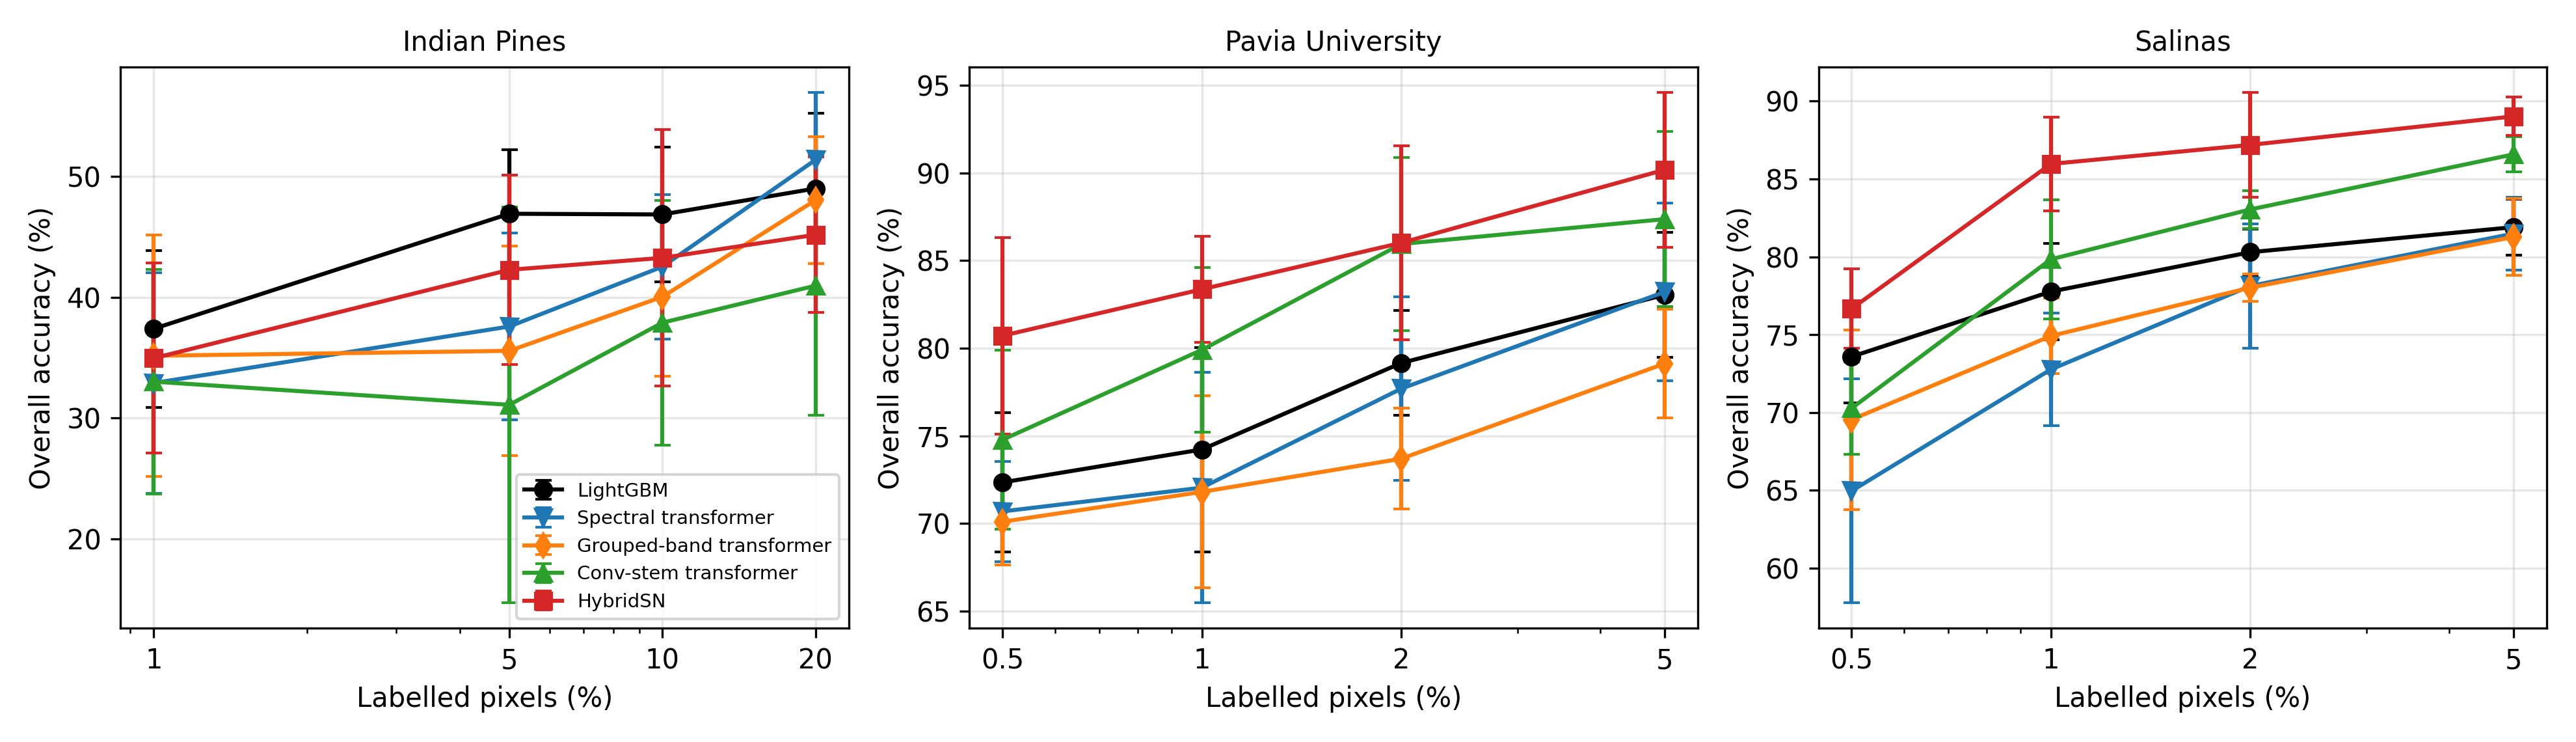
\includegraphics[width=\textwidth]{fig_scenes.png}
\caption{Overall accuracy on spatially disjoint test areas against the labelled share (mean $\pm$ SD over 5 seeds, logarithmic axis).}
\label{fig:scenes}
\end{figure}

\subsection{Local soil}
Table~\ref{tab:local} counts the budget in labelled physical samples. HybridSN has the highest mean OA at every budget and is significantly ahead of LightGBM with four samples per class ($+8.8$\pp, 95\% CI 5.0--12.6, $q=0.012$). With fewer samples its lead is 2.8--4.3\pp\ and not significant; its seed-to-seed spread is large at one sample per class ($\pm16.6$\pp). The grouped-band transformer is level with LightGBM from two samples per class ($+1.2$ to $+2.5$\pp; $q=0.052$ at four). The spectral and conv-stem transformers are unstable: in some repeats they stay near chance even with four samples per class. With one sample per class, all three transformers are significantly below LightGBM ($q\le0.035$). Two test samples per class and the confounding of class with moisture (Section~\ref{sec:data}) limit how far these figures generalise.

\begin{table}
\tbl{Local soil: overall accuracy (\%) on held-out physical samples by labelled samples per class (mean $\pm$ SD over 5 repeated sample-level splits).}
{\resizebox{\textwidth}{!}{\begin{tabular}{cccccc}
\toprule
Samples/class & LightGBM & Spectral tr. & Grouped-band tr. & Conv-stem tr. & HybridSN \\
\midrule
1 & $61.97 \pm 3.14$ & $36.05 \pm 10.15$\textsuperscript{a} & $39.56 \pm 12.81$\textsuperscript{a} & $31.55 \pm 4.82$\textsuperscript{a} & $\mathbf{64.85 \pm 16.63}$ \\
2 & $75.66 \pm 7.90$ & $69.51 \pm 13.03$ & $76.90 \pm 5.79$ & $64.19 \pm 23.25$ & $\mathbf{78.50 \pm 9.27}$ \\
3 & $82.31 \pm 8.67$ & $77.07 \pm 10.14$ & $83.93 \pm 9.24$ & $78.94 \pm 22.40$ & $\mathbf{86.64 \pm 7.64}$ \\
4 & $87.84 \pm 1.01$ & $76.43 \pm 18.45$ & $90.36 \pm 1.86$ & $70.16 \pm 32.93$ & $\mathbf{96.67 \pm 3.57}$\textsuperscript{a} \\
\bottomrule
\end{tabular}}}
\tabnote{Training uses at most 300 patches per sample (900--3\,600 patches). \textsuperscript{a}Paired difference from LightGBM significant after BH-FDR over the 16 Local tests ($q<0.05$).}
\label{tab:local}
\end{table}

\subsection{Cross-domain transfer}
Table~\ref{tab:transfer} and Figure~\ref{fig:transfer} compare pre-trained with scratch models on the same seeds. After correction, no transfer gain is significant in either direction. \emph{Local $\rightarrow$ Indian Pines:} HybridSN gains $+2.6$ to $+7.4$\pp\ ($q\ge0.27$), enough for its mean to pass LightGBM from about 6\% labelled pixels (crossover 6.2\%, 95\% CI 5.3--11.7\%), while the spectral transformer loses accuracy as the budget grows, down to $-14.9$\pp\ at 20\% ($q=0.008$). \emph{Indian Pines $\rightarrow$ Local:} with one sample per class the centre-pixel transformers gain $+13.0$ and $+20.6$\pp\ on average, but the intervals span zero. HybridSN does not gain.

\begin{table}
\tbl{Transfer gain (pre-trained minus scratch OA, pp; mean over 5 paired seeds with 95\% CI), with BH-adjusted $q$ over all 24 transfer tests.}
{\resizebox{\textwidth}{!}{\begin{tabular}{llcccc}
\toprule
Direction & Model & Budget 1 & Budget 2 & Budget 3 & Budget 4 \\
\midrule
\multirow{3}{*}{\shortstack[l]{Local $\rightarrow$ IP\\(1, 5, 10, 20\%)}}
 & HybridSN & $+2.6$ [$-7.8$, 13.0] & $+4.1$ [$-1.7$, 9.9] & $+5.3$ [$-3.3$, 13.9] & $+7.4$ [$-0.4$, 15.2] \\
 & Grouped-band tr. & $+3.2$ [$-8.4$, 14.8] & $+3.2$ [$-0.8$, 7.1] & $-0.5$ [$-5.3$, 4.4] & $-4.1$ [$-7.5$, $-0.7$] \\
 & Spectral tr. & $-3.0$ [$-12.6$, 6.6] & $-2.9$ [$-9.5$, 3.8] & $-6.1$ [$-10.3$, $-1.8$] & $-14.9$ [$-18.5$, $-11.3$]\textsuperscript{a} \\
\midrule
\multirow{3}{*}{\shortstack[l]{IP $\rightarrow$ Local\\(1--4 samples/class)}}
 & HybridSN & $-14.1$ [$-32.5$, 4.3] & $-2.5$ [$-16.8$, 11.8] & $-2.3$ [$-26.2$, 21.7] & $+0.8$ [$-3.9$, 5.4] \\
 & Grouped-band tr. & $+13.0$ [$-11.3$, 37.3] & $+2.3$ [0.6, 4.1] & $-0.1$ [$-3.3$, 3.0] & $-1.5$ [$-3.6$, 0.5] \\
 & Spectral tr. & $+20.6$ [$-7.4$, 48.5] & $+9.0$ [$-12.9$, 30.8] & $+7.6$ [$-4.2$, 19.4] & $+14.5$ [$-8.0$, 36.9] \\
\bottomrule
\end{tabular}}}
\tabnote{IP = Indian Pines. \textsuperscript{a}$q<0.05$; all other $q\ge0.16$.}
\label{tab:transfer}
\end{table}

\begin{figure}
\centering
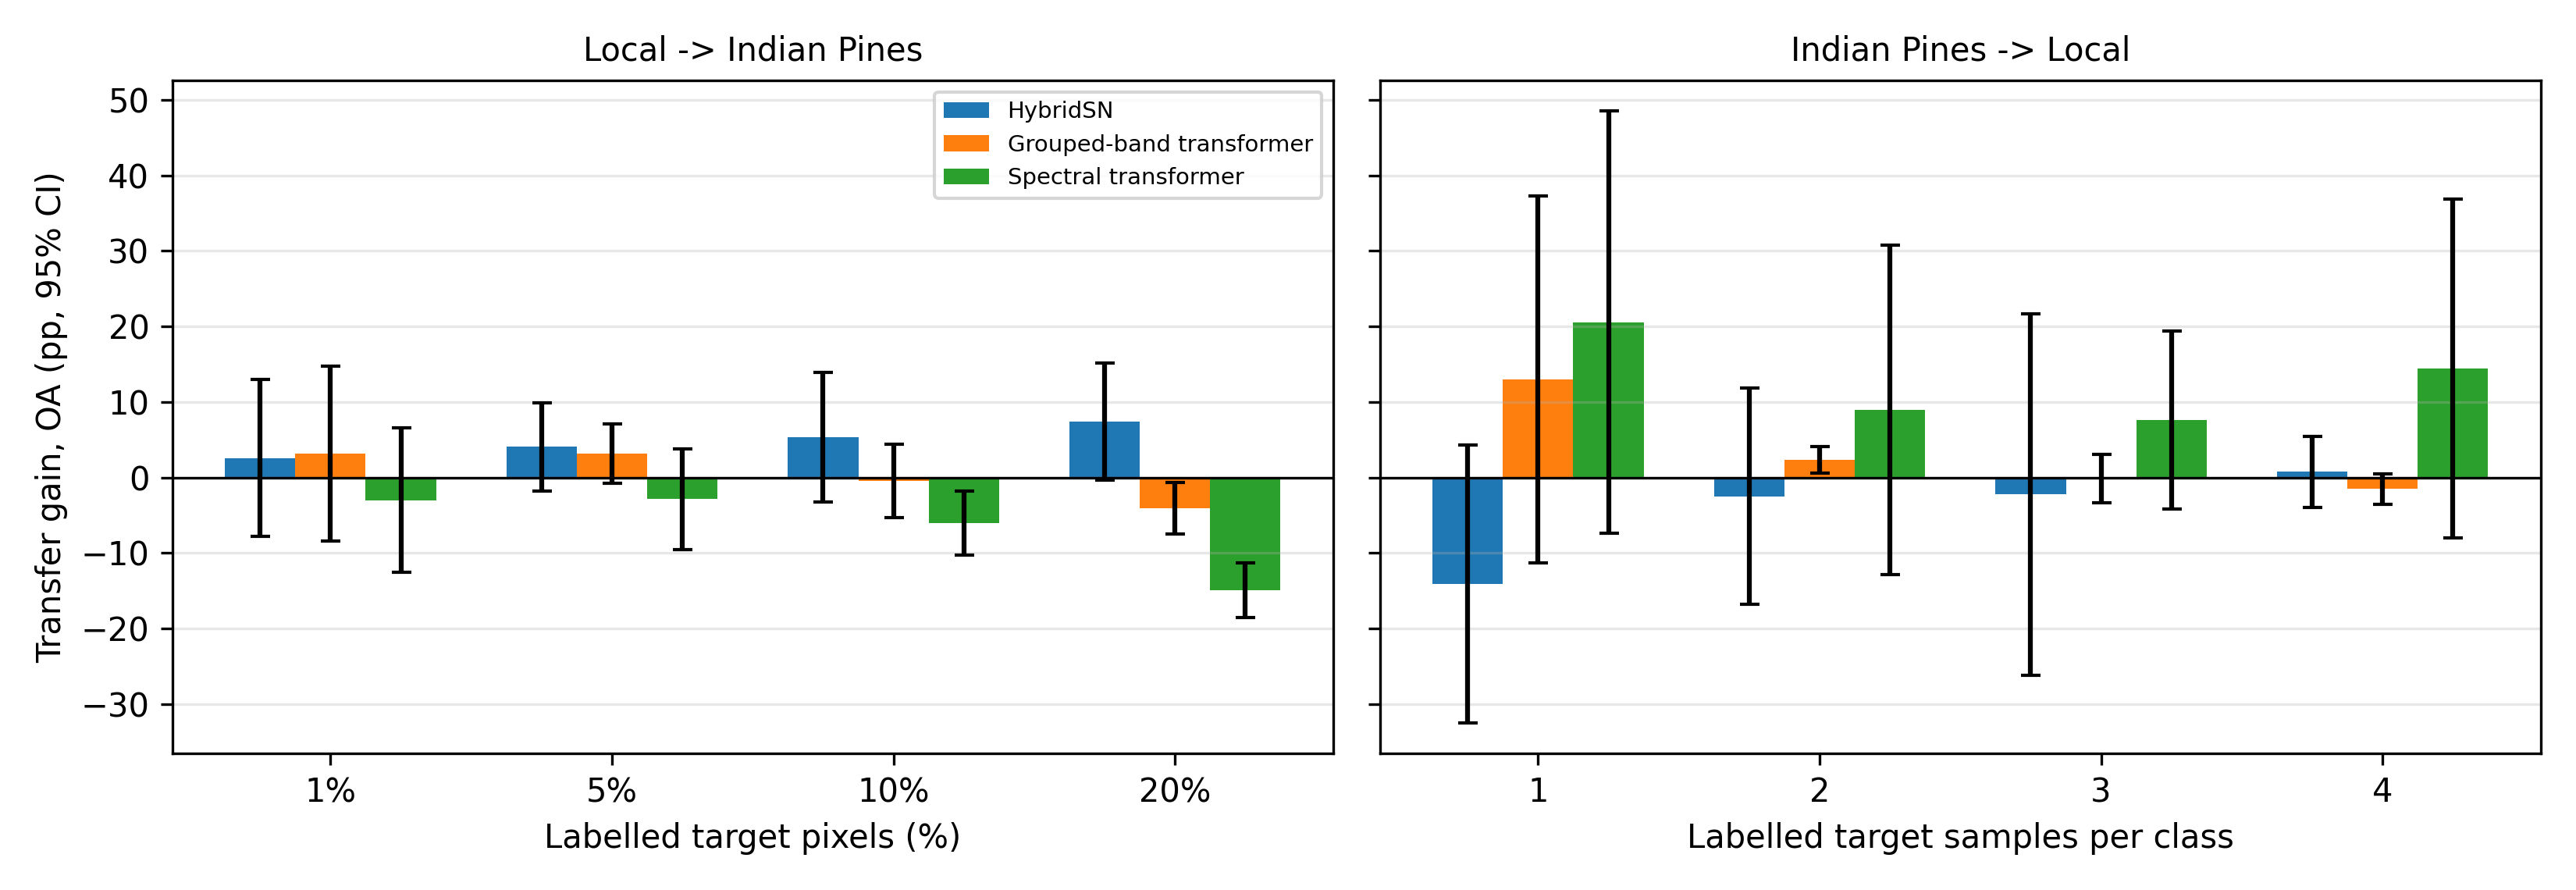
\includegraphics[width=\textwidth]{fig_transfer_gain.png}
\caption{Transfer gain (pre-trained minus scratch OA; mean and 95\% CI over 5 paired seeds) in both directions.}
\label{fig:transfer}
\end{figure}

\subsection{Band importance}
Figure~\ref{fig:shap} shows exact TreeSHAP values \citep{Lundberg2020} for LightGBM on the held-out test sets, plotted at the band centres from the sensor metadata. On the soil data (four samples per class, mean of five splits) the most influential bands are at 942\,nm, 1414\,nm and 1715\,nm. The 1414\,nm band lies on the first overtone of the O--H stretch of water and hydroxyl, and 942\,nm lies on the shoulder of the 970\,nm water band. Because soil type is confounded with moisture, this weight on water bands may reflect moisture rather than mineralogy. The 1715\,nm band is the last band of the sensor. On Indian Pines (5\% labelled, disjoint split) the top bands are at 400\,nm (the first band, where noise is high), 735\,nm (the red edge of vegetation) and 2083\,nm.

\begin{figure}
\centering
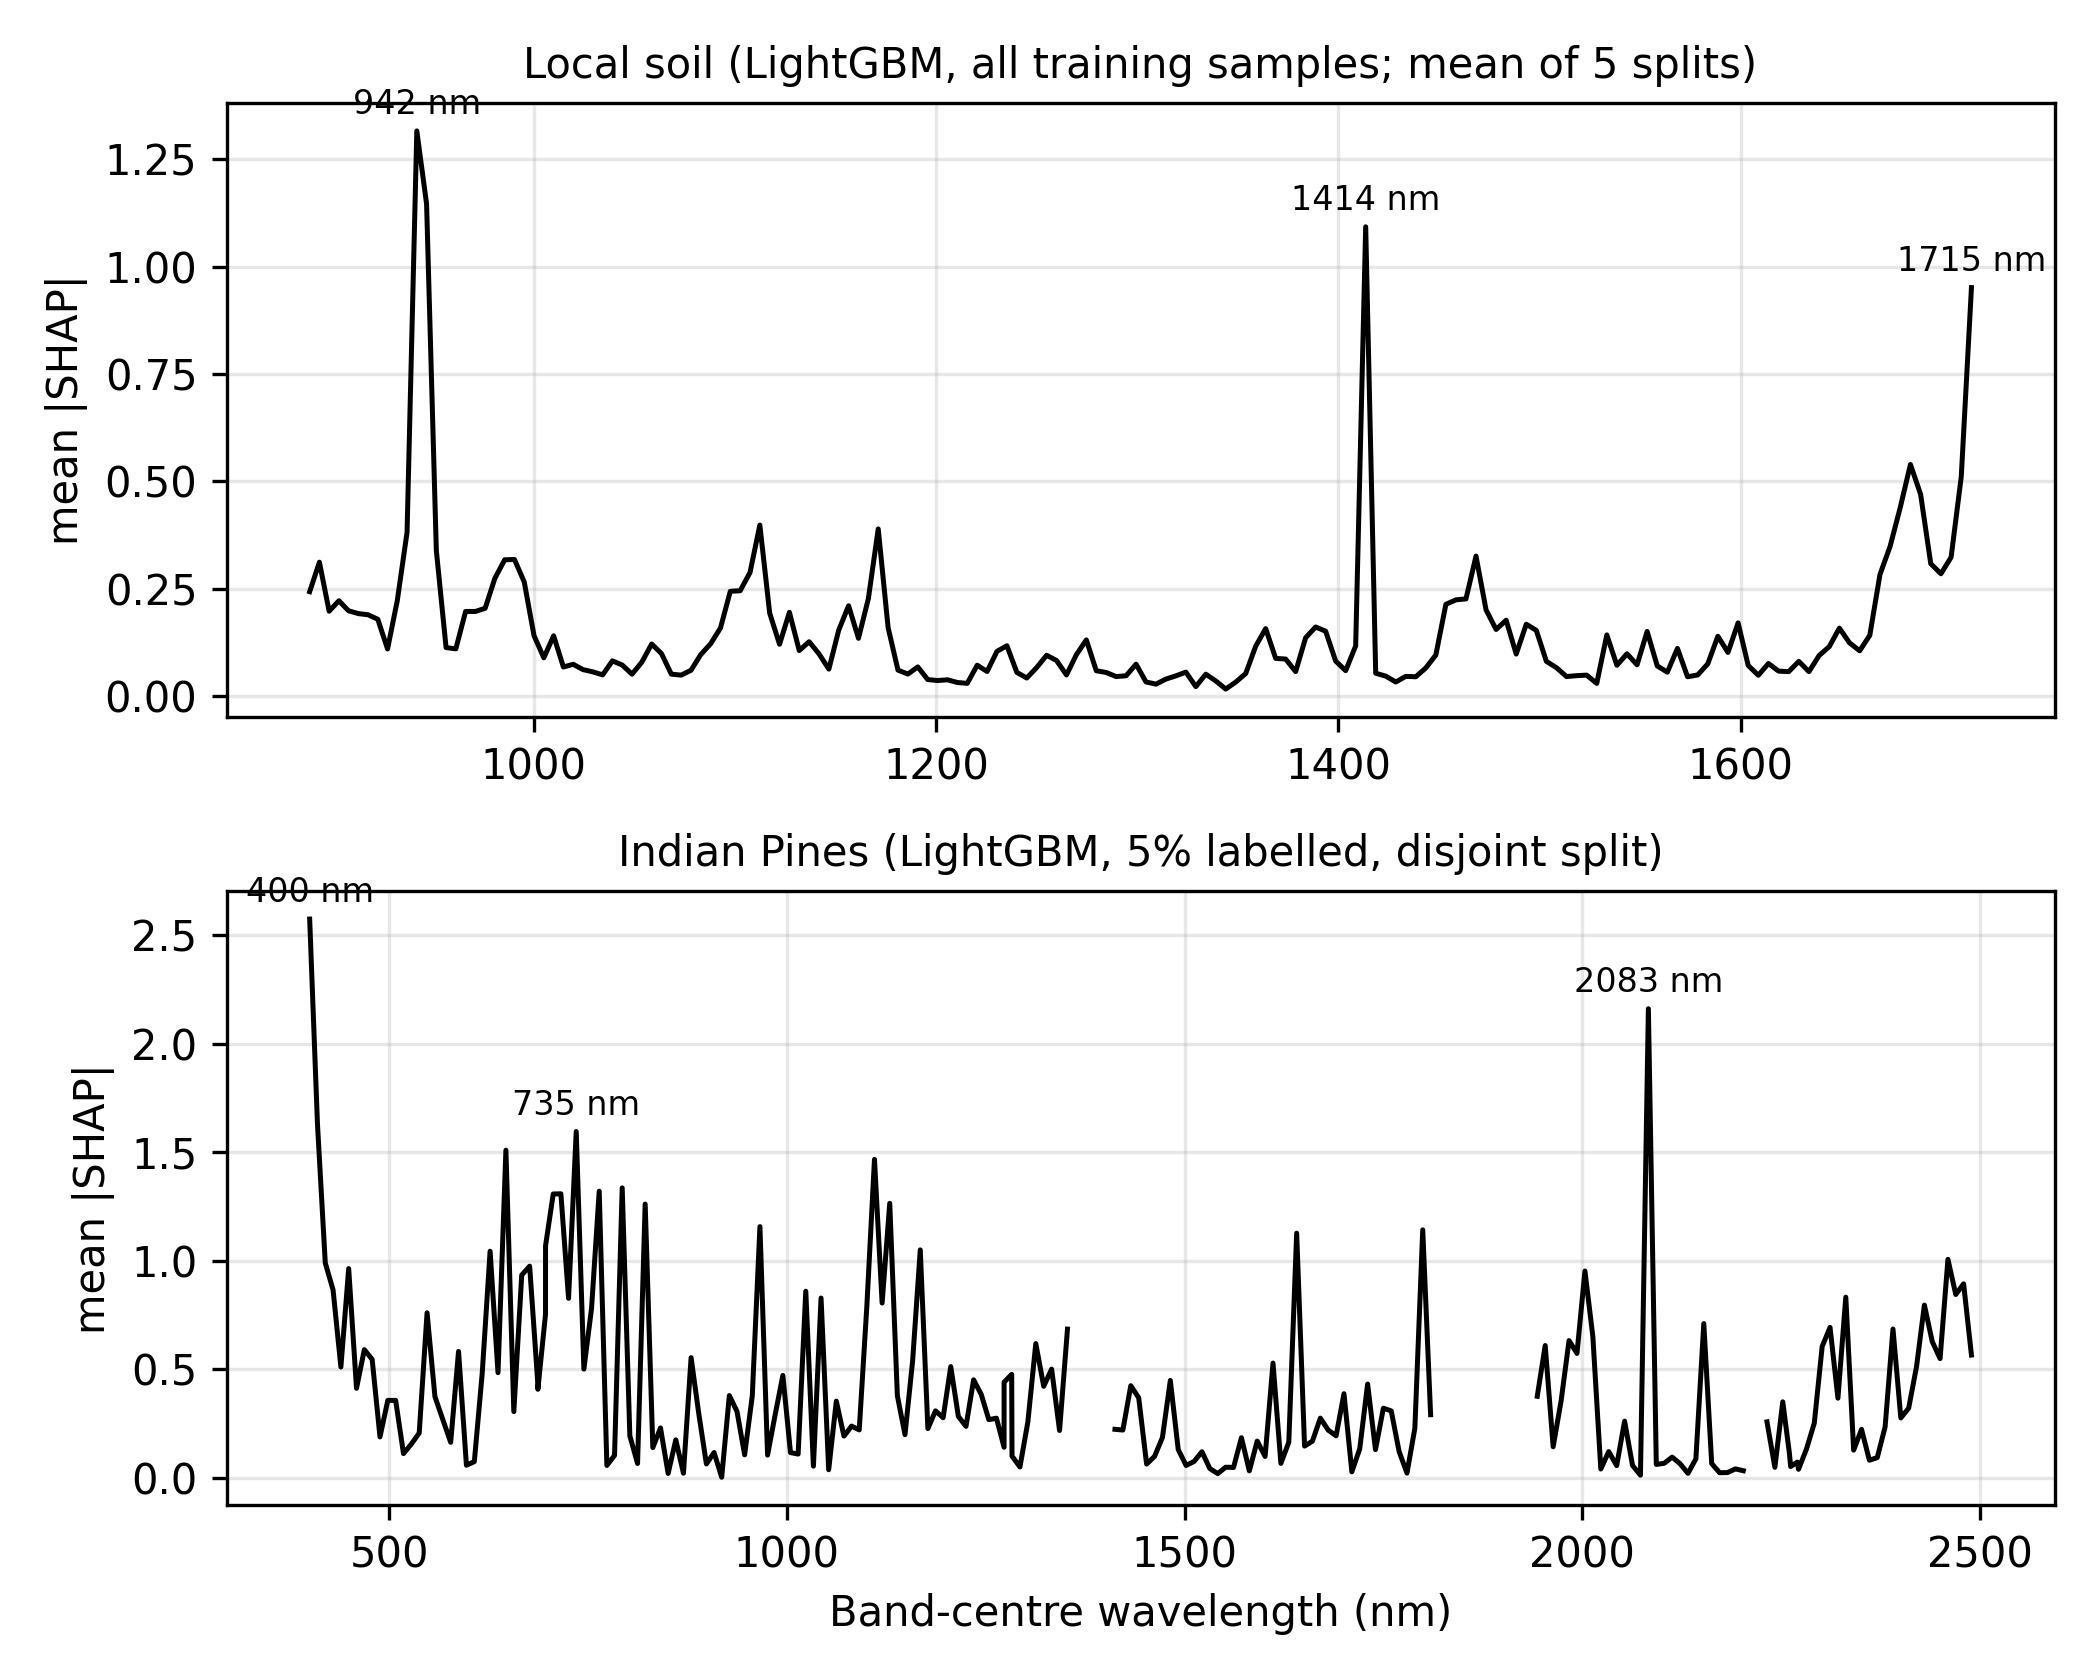
\includegraphics[width=0.85\textwidth]{fig_shap.png}
\caption{Mean absolute TreeSHAP value per band for LightGBM (summed over classes) on the held-out test sets, against band-centre wavelength from the sensor metadata. Gaps mark removed water-absorption bands.}
\label{fig:shap}
\end{figure}

\section{Discussion}\label{sec:discussion}
\emph{Local convolution matters more than the model family.} On the scenes where deep models win, the winners are the models that convolve over the patch: HybridSN, and the conv-stem transformer, which differs from the spectral transformer only by its two-layer 3-D convolutional stem. The two transformers that see only the centre spectrum were never significantly better than LightGBM. This agrees with the need of transformers for either much data or a locality prior \citep{Hassani2021}, and with the strength of tree ensembles on per-pixel input \citep{Grinsztajn2022}.

\emph{The scene matters too.} On Indian Pines, where fields are small and several classes cannot be split into disjoint areas, no deep model was significantly better than LightGBM, and all accuracies were far below published random-split figures. The disjoint split removes the overlap between training and test windows that otherwise favours patch-based models \citep{Nalepa2019}.

\emph{Transfer.} We found no transfer gain that survives correction. Pre-training on the small soil dataset reduced the accuracy of the spectral transformer on Indian Pines, whereas HybridSN's mean rose, though not significantly. Larger source datasets and more seeds would be needed to establish when cross-sensor pre-training helps.

\emph{Limitations.} The soil dataset has 24 physical samples and two test samples per class, and class is confounded with moisture and acquisition date. Five seeds give wide intervals, and many differences are not significant. All models use one training protocol without per-model tuning, and on the airborne scenes 58--85\% of deep runs reached the 50-epoch limit before early stopping, so longer training might favour the deep models. On Indian Pines, only the classes present in the training area are scored.

\section{Conclusion}
Under spatially disjoint evaluation with paired, corrected statistics, whether a deep model beats LightGBM at small annotation budgets depended on the scene and on inductive bias. HybridSN was the most accurate model on Pavia University and Salinas from 0.5\% labelled pixels, and on held-out soil samples with four labelled samples per class. On Indian Pines LightGBM was not significantly beaten. Transformers that see only the centre spectrum did not beat LightGBM significantly anywhere. In our data, LightGBM was a reasonable first baseline that needs no GPU, and 3-D convolutional models were worth trying when labels allow; cross-sensor pre-training gave no reliable gain.

\section*{Disclosure statement}
The authors report there are no competing interests to declare.

\section*{Funding}
This research received no external funding.

\section*{Data availability statement}
The Local Indian Soil images are available at \url{https://www.kaggle.com/datasets/dev123123456/local-soil-hyperspectral-dataset}. Indian Pines, Pavia University and Salinas are public benchmark scenes. Code, split definitions, seeds, per-seed results, band-centre wavelength files and run manifests are available at \url{https://github.com/Devguru-codes/research_paper_code_and_results} (folder \texttt{revision/}).

\bibliographystyle{tfcad}
\bibliography{references}

\end{document}
